% ------------------------------------------------------------------------
%                                Capítulo 4
% ------------------------------------------------------------------------
\chapter{Implementación proyecto LAGO}
% ------------------------------------------------------------------------.
\section{FPGA}

\begin{figure}[h]
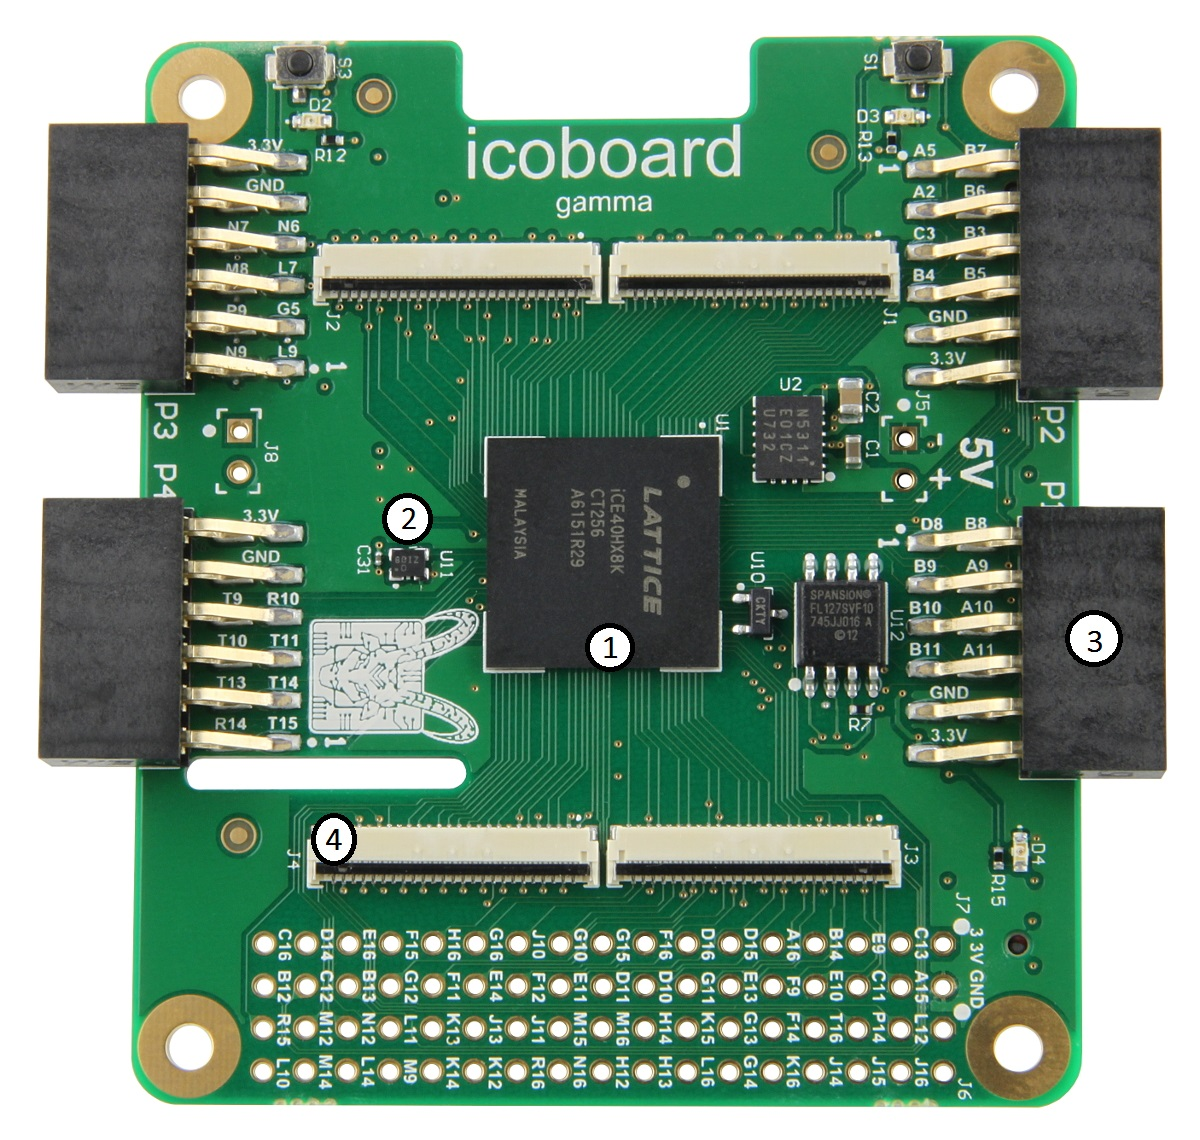
\includegraphics[scale=0.18]{Figs/icoboard.jpg} 
\centering
\caption[Icoboard con Lattice iCE40 de Trenz Electronic]{ con SRAM de 8 MBit.~\citep{IcoBoard}}
\label{icoboard}
\end{figure}

En este trabajo se selecciona la placa ICOBOARD que se muestra en la Figura~\ref{icoboard},  contiene una FPGA Lattice con 8K LUT (1), un reloj de 100 MHz (2), 8 MBit de SRAM programable en Verilog por una cadena de herramientas de código abierto, 4 conectores Pmod de 16 entradas y salidas (E/S) (3) Y 4 conectores Flat flex cada uno con 36 E/S (4). Es responsable del pre-procesamiento de los datos, el ajuste de umbrales de activación, el ajuste de los voltajes de compensación de línea base y regulación de la fuente de alto voltaje para los PMT.




La Icoboard es compatible con la Raspberry, es por medio de esta que se carga el archivo ejecutable en la FPGA. La Figura~\ref{Compatilidad} muestra un diagrama de bloques para la comunicación entre las dos tarjetas. 

\begin{figure}[h]
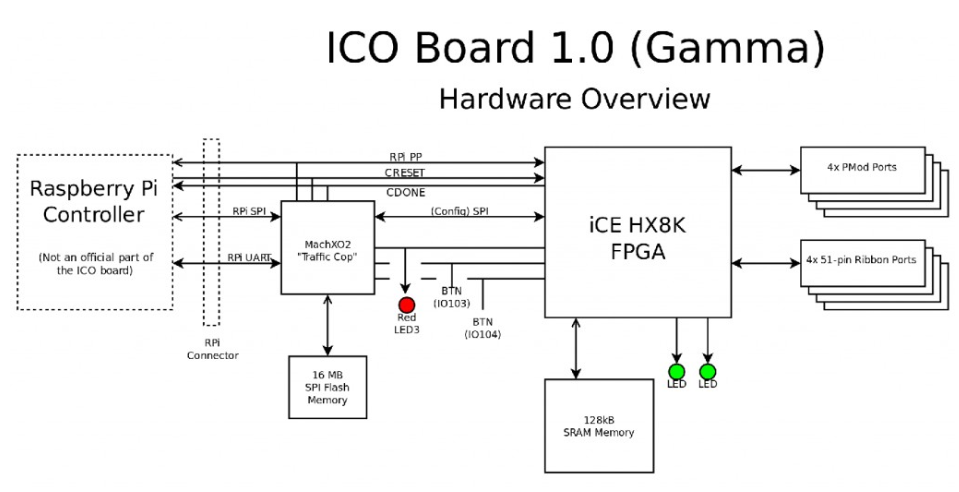
\includegraphics[width=0.93\textwidth]{Figs/icogama.PNG} 
\centering
\caption[Compatibilidad con la Raspberry]{~\citep{IcoBoard}}
\label{Compatilidad}
\end{figure}

A continuación se describe de manera detallada los recursos lógicos disponibles en la FPGA Icoboard.

La Figura~\ref{arquitectura}  muestra la arquitectura programable. La Icoboard tiene la disponibilidad de 4 bancos de puertos I/O los cuales son necesarios para la adquisición en paralelo de los 3 canales con una resolución de 12 bits, demandando una totalidad de 36 entradas. 


\begin{figure}[H]
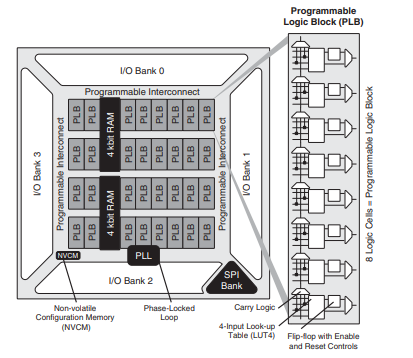
\includegraphics[scale=1.2]{Figs/architecture.PNG} 
\centering
\caption[Arquitectura iCE40]{~\citep{LatticeSemiconductor2017}}
\label{arquitectura}
\end{figure}

\noindent En la Figura~\ref{adecuacion2} se muestran los recursos lógicos disponibles para la implementación de la descripción en hardware.
Según los reportes de utilización que entrega el software utilizado Arachne, la implementación del proyecto necesita:
\begin{itemize}
    \item 38 entradas/salidas
    \item Celdas lógicas utilizadas:4335
    \item Flip Flop tipo D: 2435
\end{itemize}
Con esto se determina que la descripción en hardware necesario puede ser soportado por la FPGA seleccionada.

\begin{figure}[H]
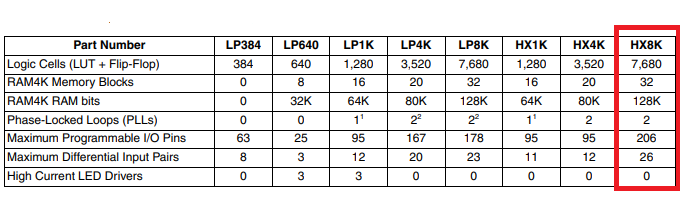
\includegraphics[width=0.93\textwidth]{Figs/tabla.png} 
\centering
\caption[Recursos lógicos de la FPGA Icoboard]{~\citep{LatticeSemiconductor2017}}
\label{adecuacion2}
\end{figure}


\section{Sensores adicionales}
En esta sección se describen los sensores usados para el proyecto, los cuales son de vital importancia para los análisis posterior del archivo de salida. El sensor de temperatura y presión barométrica permite conocer las condiciones atmósfericas básicas bajo las cuales trabaja el WCD, y de esta manera, se obtiene información de las variaciones de temperatura que afectan el comportamiento del detector y por tanto generar alteraciones en la tasa de eventos registrados.

Por otra parte, el GPS seleccionado (Adafruit Ultimate) permite conocer las condiciones de geoposicionamiento del detector, además permite la sincronización temporal de la interfaz digital al usar la señal PPS (Pulse-Per-Second).

A continuación se muestra las características más relevantes de los sensores usados.

\subsection{GPS}
Un criterio importante para la configuración entre Raspberry-GPS-FPGA es la necesidad de generar un archivo de salida de datos como se planteo en los objetivos que contenga una referencia temporal precisa, para relizar estudios dinámicos.
También, la información de geoposicionamiento del flujo de rayos cósmicos secudarios es un factor relevante que afecta el flujo de partículas detectadas con parámetros como la altura a nivel del mar y la latitud.

Es importante que el GPS seleccionado tenga la señal PPS (Pulse-Per-Second) como uno de sus periféricos. 
Esta señal y el tiempo UTC del GPS proporcionan la información de tiempo a la Raspberry Pi.

Dentro las características más relevantes del GPS está el periférico PPS, Y una interfaz de comunicación UART a 9600 baud.

\begin{figure}[H]
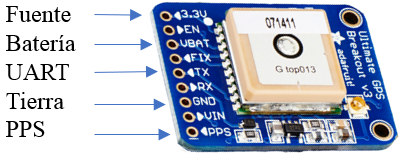
\includegraphics[scale=0.85]{Figs/gps.png} 
\centering
\caption[GPS adafruit ultimate]{~\citep{Adafruit2020}}
\label{adecuacion}
\end{figure}

\subsection{Temperatura y presión atmosférica}
El sensor de temperatura y presión utilizado cuenta con una interfaz de comunicación I2C, un convertidor análogo digital con 16 bits de resolución que proporciona datos de la presión y la temperatura. 
El sensor es calibrado por el fabricante almacenando 11 coeficientes únicos en el chip, los cuales se usan en la lectura de presión y temperatura. 
Este dispositivo opera con 3V, una corriente de 500uA durante la conversión y 1uA en reposo.

\begin{figure}[H]
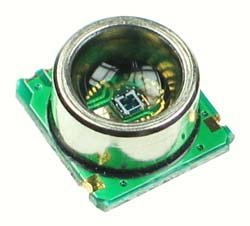
\includegraphics[scale=0.7]{Figs/hp03s.jpg} 
\centering
\caption[Sensor HP03S de presión y temperatura]{ ~\citep{HP03SDatasheet}}
\label{adecuacion}
\end{figure}

\begin{figure}[H]
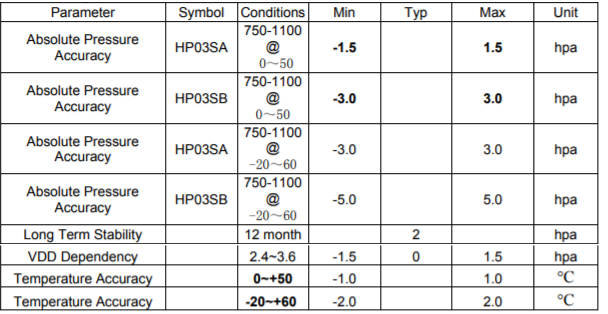
\includegraphics[width=0.93\textwidth]{Figs/tabla_hp03s.PNG} 
\centering
\caption[Características de salida del sensor de presión y temperatura]{ ~\citep{HP03SDatasheet}}
\label{adecuacion}
\end{figure}



\section{Raspberry Pi B+}
Se eligió la Raspberry Pi 3 Model B+ puesto que esta cumple con los requerimientos necesarios para el desarrollo del proyecto.
%y además existían unidades en el grupo Halley.

\begin{table}[h] 
\begin{center}
\begin{tabular}{|p{4cm}|p{10cm}|}\hline
%\rowcolor[HTML]{FFFFC7} 
%\multicolumn{2}{|c|} {RASPBERRY PI 3 MODEL B+}\\ \hline  
\textbf{Procesador} & Broadcom BCM2837B0, Cortex-A53 (ARMv8) 64-bit SoC\\ \hline
\textbf{Frecuencia de reloj}& 1,4 GHz\\ \hline
\textbf{Memoria}    & 1GB LPDDR2 SDRAM\\ \hline
\textbf{Conectividad inalámbrica} & 2.4GHz / 5GHz IEEE 802.11.b/g/n/ac Bluetooth 4.2, BLE\\ \hline
\textbf{Conectividad de red} & Gigabit Ethernet over USB 2.0 (300 Mbps de máximo teórico)\\ \hline 
\textbf{Puertos}    & GPIO 40 pines, HDMI, 4 x USB 2.0, CSI (cámara Raspberry Pi), DSI (pantalla tácil), Toma auriculares / vídeo compuesto, Micro SD, Micro USB (alimentación), Power-over-Ethernet (PoE)\\ \hline
\end{tabular}
\caption{Características Raspberry Pi 3 Model B+~\citep{Pasor2018}}
\label{tabla2}
\end{center}
\end{table}

Sus características más destacadas se muestran en la Tabla~\ref{tabla2}. Tiene una frecuencia de 1,4 GHz para sus cuatro núcleos  ayudando a obtener mejores rendimientos en muchas de las tareas que se propongan a este miniPC. 
La plataforma soporta diversos sistemas operativos, desde GNU/Linux hasta algunas versiones de Windows, para el caso del proyecto se utiliza Raspian (distribución de GNU/Linux basado en Debian para Raspberry PI).

Uno de los retos que se presentan en el desarrollo del proyecto es adquirir los datos de interés y almacenarlos, por esta razón se utilizaron librerías que permiten el uso de pines GPIO (General Purpose Input Output) con el lenguaje de medio nivel (C o C++) y Python, esto con el fin de hacer uso eficiente de los recursos del sistema.
%, de tal manera que el procesador no se ocupe en procesos innecesarios.


\section{Integración de periféricos}
Este circuito se implementa para tener la conexión de la Raspberry y la FPGA con los periféricos de una manera más organizada y así lograr la comunicación de todos los componentes utilizados en el proyecto.

La PCB se diseña a doble capa, esta es compatible con una amplia gama de Raspberry y tiene dimensiones de 56.4 x 65.9 mm.
Ver Figura~\ref{pcb}.

\begin{figure}[H]
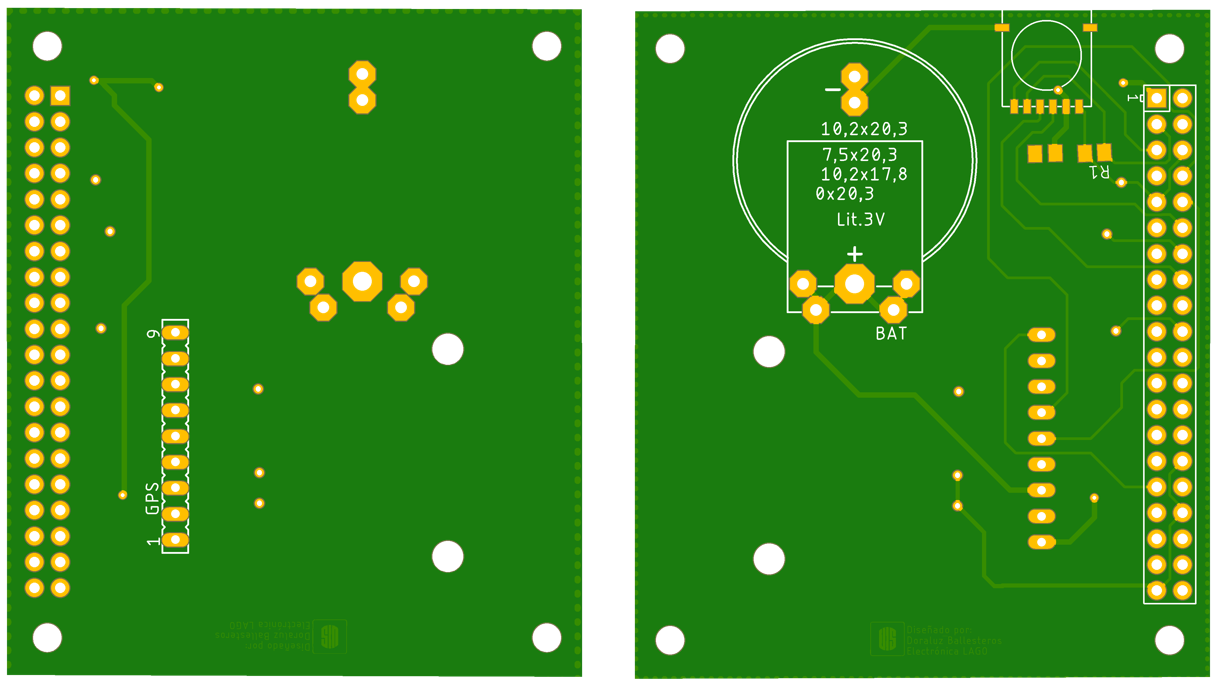
\includegraphics[width=0.90\textwidth]{Figs/pcb_eagle.PNG} 
\centering
\caption{Diseño de la PCB}
\label{pcb}
\end{figure}

En la Figura~\ref{pcb} se muestra una tarjeta ''shield'' donde se realiza la comunicación teniendo en cuenta cada uno de los protocolos que permiten recibir la información suministrada por los sensores.
En la PCB diseñada se realizaron conexiones del protocolo UART para el GPS Adafruit Ultimate e I2C para el sensor de presión y temperatura HP03S con pines de la Raspberry pi3 B+. 

\begin{figure}[H]
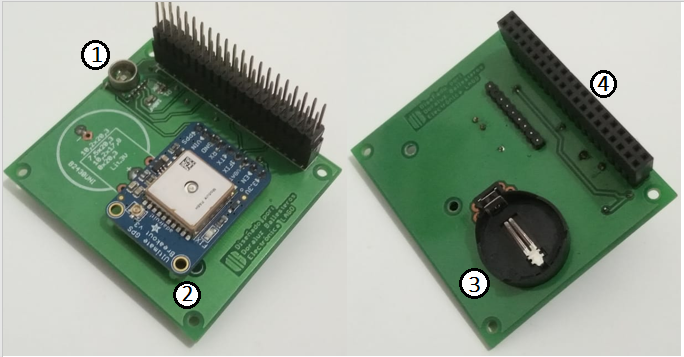
\includegraphics[width=0.85\textwidth]{Figs/pcb.PNG} 
\centering
\caption{PCB de integración de periféricos}
\label{pcb}
\end{figure}

Se integran los perifericos captadores así: sensor HP03S (1), GPS Adafruit Ultimate (2), batería (3), conector 40 pines (4).

\begin{figure}[H]
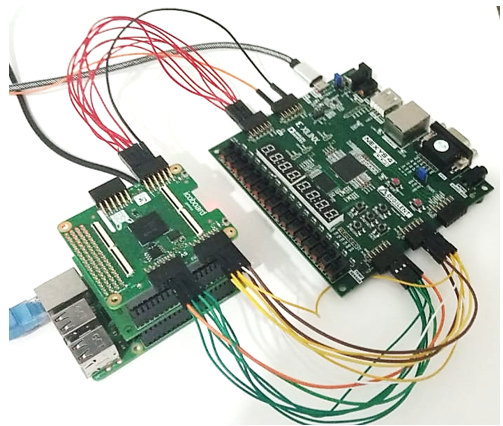
\includegraphics[scale=0.75]{Figs/lagofinal.PNG} 
\centering
\caption{Implementación proyecto LAGO para pruebas con nexys 4-DDR}
\label{nexys}
\end{figure}
En la Figura~\ref{nexys} se puede observar la conexión implementada para simular la señales provenietes de la tarjeta digitalizadora presentada en la Figura~\ref{sistema}  por medio de una Nexys 4-DDR.


\begin{figure}[H]
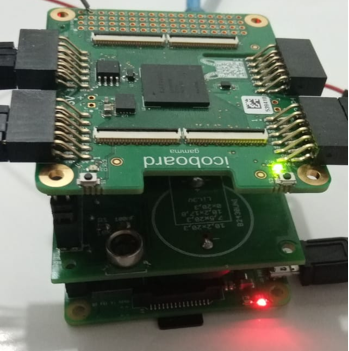
\includegraphics[scale=0.85]{Figs/icoboardfinal.PNG}
\centering
\caption{Implementación del hardware LAGO actualizado}
\label{lagofin}
\end{figure}

En la Figura~\ref{lagofin} se encuentra ubicado de abajo hacia arriba la Raspberry Pi model B+, PCB con perifericos y la FPGA Icoboard.

Note que la Raspberry alimenta a todo el cojunto de tarjetas, esta entrega una tensión de 3,3 V.

%\begin{figure}[H]
%\includegraphics[scale=0.2]{Figs/P1070196.JPG} 
%\centering
%\caption{Implementación proyecto LAGO original }
%\label{original}
%\end{figure}

%Finalmente se implementa e
El diseño final del sistema de adquisición se muestra en la Figura~\ref{lagofin}, nótese que se ve mucho más compacto  que el LAGO original Figura~\ref{adecuacion}, excepto por nexys 4-DDR usada como hardware externo para las pruebas Figura~\ref{nexys}.

% ------------------------------------------------------------------------